% questions.tex —— 2017 年·北京卷·理科 · 题目内容片段（无答案）
% 由 tools/generate_projects.py 依来源总账自 2017/2017_数学真题_北京理_试题.md 生成，勿手改（改源 MD 后重跑）

\gkpart{数学}

\begin{gktip}
\textbf{来源说明}：本题面依据固定源 PDF 两页 A3 页面逐题核对，原卷印刷页码 1031–1032。固定源不附答案；本文件仅为题面规范源。
\end{gktip}

\gkpart{一、选择题}

\begin{question}
\gkti{1}
若集合 $A=\{x\mid -2<x<1\}$，$B=\{x\mid x<-1\text{ \text{或} }x>3\}$，则 $A\cap B=$（　）

\begin{itemize}
\item （A）$\{x\mid -2<x<-1\}$
\item （B）$\{x\mid -2<x<3\}$
\item （C）$\{x\mid -1<x<1\}$
\item （D）$\{x\mid 1<x<3\}$
\end{itemize}

\end{question}
\begin{question}
\gkti{2}
若复数 $(1-\mathrm i)(a+\mathrm i)$ 在复平面内对应的点在第二象限，则实数 $a$ 的取值范围是（　）

\begin{itemize}
\item （A）$(-\infty,1)$
\item （B）$(-\infty,-1)$
\item （C）$(1,+\infty)$
\item （D）$(-1,+\infty)$
\end{itemize}

\Needspace{0.4\textheight}
\end{question}
\begin{question}
\gkti{3}
执行如图所示的程序框图，输出的 $S$ 值为（　）
\nopagebreak[4]
\begin{center}\begin{tikzpicture}[>=stealth,thick,
  term/.style={draw,rounded corners=3pt,minimum width=22mm,minimum height=7mm},
  proc/.style={draw,minimum width=30mm,minimum height=8mm,align=center},
  test/.style={draw,diamond,aspect=2.2,inner sep=1pt,align=center},
  io/.style={draw,trapezium,trapezium left angle=70,trapezium right angle=110,
    minimum width=27mm,minimum height=8mm,align=center}]
  \node[term] (start) at (-2,0) {开始};
  \node[proc] (init) at (-2,-1.15) {$k=0,\ s=1$};
  \node[test] (test) at (0,-2.65) {$k<3$？};
  \node[proc] (inc) at (3,-2.65) {$k=k+1$};
  \node[proc] (update) at (3,-1.15) {$s=\dfrac{s+1}{s}$};
  \node[io] (out) at (0,-4.15) {输出 $s$};
  \node[term] (stop) at (0,-5.25) {结束};
  \draw[->] (start)--(init);
  \draw[->] (init)--(test);
  \draw[->] (test.east)--node[above]{是}(inc.west);
  \draw[->] (inc.north)--(update.south);
  \draw[->] (update.west)--++(-1.05,0)|-(test.north);
  \draw[->] (test.south)--node[right]{否}(out.north);
  \draw[->] (out)--(stop);
\end{tikzpicture}
\end{center}
\nopagebreak[4]
\begin{itemize}
\item （A）$2$
\item （B）$\dfrac32$
\item （C）$\dfrac53$
\item （D）$\dfrac85$
\end{itemize}

\end{question}
\begin{question}
\gkti{4}
\Needspace{5\baselineskip}
若 $x,y$ 满足

\nopagebreak[4]
\[
\begin{cases}
x\leqslant3,\\
x+y\geqslant2,\\
y\leqslant x,
\end{cases}
\]

则 $x+2y$ 的最大值为（　）

\begin{itemize}
\item （A）$1$
\item （B）$3$
\item （C）$5$
\item （D）$9$
\end{itemize}

\end{question}
\begin{question}
\gkti{5}
已知函数 $f(x)=3^x-\left(\dfrac13\right)^x$，则 $f(x)$（　）

\begin{itemize}
\item （A）是奇函数，且在 $\mathbb R$ 上是增函数
\item （B）是偶函数，且在 $\mathbb R$ 上是增函数
\item （C）是奇函数，且在 $\mathbb R$ 上是减函数
\item （D）是偶函数，且在 $\mathbb R$ 上是减函数
\end{itemize}

\end{question}
\begin{question}
\gkti{6}
设 $\boldsymbol m,\boldsymbol n$ 为非零向量，则“存在负数 $\lambda$，使得 $\boldsymbol m=\lambda\boldsymbol n$”是“$\boldsymbol m\cdot\boldsymbol n<0$”的（　）

\begin{itemize}
\item （A）充分而不必要条件
\item （B）必要而不充分条件
\item （C）充分必要条件
\item （D）既不充分也不必要条件
\end{itemize}

\Needspace{0.4\textheight}
\end{question}
\begin{question}
\gkti{7}
某四棱锥的三视图如图所示，则该四棱锥的最长棱的长度为（　）
\nopagebreak[4]
\begin{center}\begin{tikzpicture}[thick,>=stealth,line cap=round,line join=round,
  dim/.style={<->,thin}, every node/.style={font=\small}]
  % Front view: right triangle with horizontal and vertical legs both 2.
  \draw (0,0)--(2.4,0)--(2.4,2.4)--cycle;
  \draw[dim] (0,-.42)--(2.4,-.42) node[midway,below]{2};
  \draw[thin] (0,-.12)--(0,-.52) (2.4,-.12)--(2.4,-.52);
  \draw[dim] (2.82,0)--(2.82,2.4) node[midway,right]{2};
  \draw[thin] (2.52,0)--(2.92,0) (2.52,2.4)--(2.92,2.4);
  \node at (1.2,2.85) {正视图};
  % Side view: square face and its visible diagonal.
  \draw (5,0) rectangle (7.4,2.4);
  \draw (5,0)--(7.4,2.4);
  \draw[dim] (5,-.42)--(7.4,-.42) node[midway,below]{2};
  \draw[thin] (5,-.12)--(5,-.52) (7.4,-.12)--(7.4,-.52);
  \node at (6.2,2.85) {侧视图};
  % Plan view: right triangle and its internal diagonal.
  \draw (0,-3.15)--(2.4,-3.15)--(2.4,-5.55)--cycle;
  \draw (0,-3.15)--(2.4,-5.55);
  \node at (1.2,-5.95) {俯视图};
\end{tikzpicture}
\end{center}
\nopagebreak[4]
\begin{itemize}
\item （A）$3\sqrt2$
\item （B）$2\sqrt3$
\item （C）$2\sqrt2$
\item （D）$2$
\end{itemize}

\end{question}
\begin{question}
\gkti{8}
根据有关资料，围棋状态空间复杂度的上限 $M$ 约为 $3^{361}$，而可观测宇宙中普通物质的原子总数 $N$ 约为 $10^{80}$，则下列各数中与 $\dfrac MN$ 最接近的是（　）

（参考数据：$\lg3\approx0.48$）

\begin{itemize}
\item （A）$10^{33}$
\item （B）$10^{53}$
\item （C）$10^{73}$
\item （D）$10^{93}$
\end{itemize}

\end{question}
\gkpart{二、填空题}

\begin{question}
\gkti{9}
若双曲线 $x^2-\dfrac{y^2}{m}=1$ 的离心率为 $\sqrt3$，则实数 $m=$\gkblank{}。

\end{question}
\begin{question}
\gkti{10}
若等差数列 $\{a_n\}$ 和等比数列 $\{b_n\}$ 满足 $a_1=b_1=-1$，$a_4=b_4=8$，则 $\dfrac{a_2}{b_2}=$\gkblank{}。

\end{question}
\begin{question}
\gkti{11}
在极坐标系中，点 $A$ 在圆 $\rho^2-2\rho\cos\theta-4\rho\sin\theta+4=0$ 上，点 $P$ 的坐标为 $(1,0)$，则 $|AP|$ 的最小值为\gkblank{}。

\end{question}
\begin{question}
\gkti{12}
在平面直角坐标系 $xOy$ 中，角 $\alpha$ 与角 $\beta$ 均以 $Ox$ 为始边，它们的终边关于 $y$ 轴对称，若 $\sin\alpha=\dfrac13$，则 $\cos(\alpha-\beta)=$\gkblank{}。

\end{question}
\begin{question}
\gkti{13}
能够说明“设 $a,b,c$ 是任意实数。若 $a>b>c$，则 $a+b>c$”是假命题的一组整数 $a,b,c$ 的值依次为\gkblank{}。

\Needspace{0.4\textheight}
\end{question}
\begin{question}
\gkti{14}
三名工人加工同一种零件，他们在一天中的工作情况如图所示，其中 $A_i$ 的横、纵坐标分别为第 $i$ 名工人上午的工作时间和加工的零件数，点 $B_i$ 的横、纵坐标分别为第 $i$ 名工人下午的工作时间和加工的零件数，$i=1,2,3$。
\nopagebreak[4]
\begin{center}\begin{tikzpicture}[x=5cm,y=3.4cm,>=stealth,thick,
  every node/.style={font=\small}]
  \draw[->] (0,0)--(1.08,0) node[right]{工作时间（小时）};
  \draw[->] (0,0)--(0,1.08) node[above]{零件数（件）};
  \node[below left] at (0,0) {$O$};
  \foreach \x/\y/\lab/\pos in {
    .34/.84/$A_1$/above left,
    .14/.33/$A_2$/left,
    .37/.09/$A_3$/below,
    .75/.20/$B_1$/below,
    .67/.55/$B_2$/above left,
    .91/.63/$B_3$/above right}
    {\fill (\x,\y) circle (1.2pt);\node[\pos] at (\x,\y) {\lab};}
\end{tikzpicture}
\end{center}
\nopagebreak[4]
(1) 记 $Q_i$ 为第 $i$ 名工人在这一天中加工的零件总数，则 $Q_1,Q_2,Q_3$ 中最大的是\gkblank{}；

(2) 记 $p_i$ 为第 $i$ 名工人在这一天中平均每小时加工的零件数，则 $p_1,p_2,p_3$ 中最大的是\gkblank{}。

\end{question}
\gkpart{三、解答题}

\begin{question}
\gkti{15}
在 $\triangle ABC$ 中，$\angle A=60^\circ$，$c=\dfrac37a$。

(1) 求 $\sin C$ 的值；

(2) 若 $a=7$，求 $\triangle ABC$ 的面积。

\Needspace{0.4\textheight}
\end{question}
\begin{question}
\gkti{16}
如图，在四棱锥 $P-ABCD$ 中，底面 $ABCD$ 为正方形，平面 $PAD\perp$ 平面 $ABCD$，点 $M$ 在线段 $PB$ 上，$PD\parallel$ 平面 $MAC$，$PA=PD=\sqrt6$，$AB=4$。

(1) 求证：$M$ 为 $PB$ 的中点；

(2) 求二面角 $B-PD-A$ 的大小；

(3) 求直线 $MC$ 与平面 $BDP$ 所成角的正弦值。
\nopagebreak[4]
\begin{center}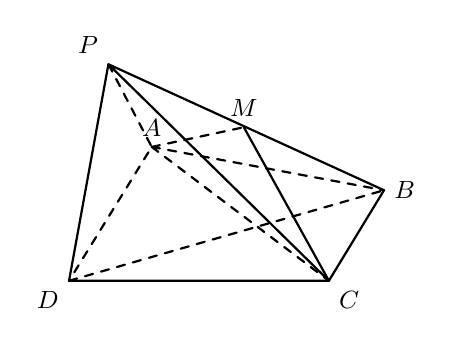
\begin{tikzpicture}[thick,line cap=round,line join=round,
  every node/.style={font=\small}]
  \coordinate (P) at (0,2.75);
  \coordinate (D) at (-.5,0);
  \coordinate (C) at (2.8,0);
  \coordinate (B) at (3.5,1.15);
  \coordinate (A) at (.55,1.7);
  \coordinate (M) at (1.72,1.95);
  \draw (P)--(D)--(C)--(B)--(P)--(C);
  \draw (M)--(C);
  \draw[dashed] (P)--(A)--(D) (A)--(B) (A)--(C) (A)--(M) (D)--(B);
  \node[above left] at (P) {$P$};
  \node[above] at (A) {$A$};
  \node[right] at (B) {$B$};
  \node[below right] at (C) {$C$};
  \node[below left] at (D) {$D$};
  \node[above] at (M) {$M$};
\end{tikzpicture}
\end{center}
\nopagebreak[4]
\Needspace{0.4\textheight}
\end{question}
\begin{question}
\gkti{17}
为了研究一种新药的疗效，选 $100$ 名患者随机分成两组，每组各 $50$ 名，一组服药，另一组不服药。一段时间后，记录了两组患者的生理指标 $x$ 和 $y$ 的数据，并制成如图，其中“$\ast$”表示服药者，“$+$”表示未服药者。
\nopagebreak[4]
\begin{center}\begin{tikzpicture}[x=4.7cm,y=.048cm,>=stealth,thick,
  every node/.style={font=\small}]
  \draw[->] (0,35)--(1.08,35) node[right]{指标 $x$};
  \draw[->] (0,35)--(0,104) node[above]{指标 $y$};
  \node[below left] at (0,35) {$O$};
  \draw[dashed] (0,60)--(1.02,60);
  \draw[dashed] (.55,35)--(.55,101);
  \node[left] at (0,60) {$60$};
  \node[below] at (.55,35) {$1.7$};
  % Schematic symbol positions only: the source provides no individual data
  % coordinates. Fifty marks per group retain the source's visible count.
  \foreach \x/\y in {
    .12/89,.16/84,.20/78,.24/72,.28/65,.32/91,.36/83,.40/76,.44/69,.48/63,
    .10/58,.14/55,.18/52,.22/49,.26/46,.30/43,.34/40,.38/37,.42/34,.46/31,
    .18/88,.24/82,.30/75,.36/68,.42/61,.48/86,.50/79,.52/73,.54/66,.58/59,
    .08/95,.15/93,.23/90,.31/88,.39/85,.47/82,.11/75,.19/72,.27/70,.35/67,
    .43/64,.09/54,.17/51,.25/48,.33/45,.41/42,.49/39,.13/36,.21/33,.29/30}
    \node at (\x,\y) {$\ast$};
  \foreach \x/\y in {
    .57/86,.62/83,.67/80,.72/77,.77/74,.82/71,.87/68,.92/65,.97/62,.60/94,
    .65/91,.70/88,.75/85,.80/82,.85/79,.90/76,.95/73,.59/69,.64/66,.69/63,
    .74/60,.79/58,.84/56,.89/54,.94/52,.98/50,.61/97,.68/95,.76/93,.83/90,
    .91/88,.57/84,.63/81,.71/78,.78/75,.86/72,.93/70,.60/67,.67/64,.75/61,
    .82/59,.90/57,.96/55,.58/53,.66/51,.73/49,.81/47,.88/45,.95/43,.99/40}
    \node at (\x,\y) {$+$};
  \node[above left] at (.72,96) {$A$};
  \node[above left] at (.32,78) {$B$};
  \node[above right] at (.98,68) {$C$};
  \node[above left] at (.24,72) {$D$};
\end{tikzpicture}
\end{center}
\nopagebreak[4]
(1) 从服药的 $50$ 名患者中随机选出一人，求此人指标 $y$ 的值小于 $60$ 的概率；

(2) 从图中 $A,B,C,D$ 四人中随机选出两人，记 $\xi$ 为选出的两人中指标 $x$ 的值大于 $1.7$ 的人数，求 $\xi$ 的分布列和数学期望 $E(\xi)$；

(3) 试判断这 $100$ 名患者中服药者指标 $y$ 数据的方差与未服药者指标 $y$ 数据的方差的大小。（只需写出结论）

\end{question}
\begin{question}
\gkti{18}
已知抛物线 $C:y^2=2px$ 过点 $P(1,1)$。过点 $\left(0,\dfrac12\right)$ 作直线 $l$ 与抛物线 $C$ 交于不同的两点 $M,N$，过点 $M$ 作 $x$ 轴的垂线分别与直线 $OP,ON$ 交于点 $A,B$，其中 $O$ 为原点。

(1) 求抛物线 $C$ 的方程，并求其焦点坐标和准线方程；

(2) 求证：$A$ 为线段 $BM$ 的中点。

\end{question}
\begin{question}
\gkti{19}
已知函数 $f(x)=\mathrm e^x\cos x-x$。

(1) 求曲线 $y=f(x)$ 在点 $(0,f(0))$ 处的切线方程；

(2) 求函数 $f(x)$ 在区间 $\left[0,\dfrac\pi2\right]$ 上的最大值和最小值。

\end{question}
\begin{question}
\gkti{20}
\Needspace{5\baselineskip}
设 $\{a_n\}$ 和 $\{b_n\}$ 是两个等差数列，记

\nopagebreak[4]
\[
c_n=\max\{b_1-a_1n,\ b_2-a_2n,\ \cdots,\ b_n-a_nn\}\qquad(n=1,2,3,\cdots),
\]

其中 $\max\{x_1,x_2,\cdots,x_s\}$ 表示 $x_1,x_2,\cdots,x_s$ 这 $s$ 个数中最大的数。

(1) 若 $a_n=n$，$b_n=2n-1$，求 $c_1,c_2,c_3$ 的值，并证明 $\{c_n\}$ 是等差数列；

(2) 证明：或者对任意正数 $M$，存在正整数 $m$，当 $n\geqslant m$ 时，$\dfrac{c_n}{n}>M$；或者存在正整数 $m$，使得 $c_m,c_{m+1},c_{m+2},\cdots$ 是等差数列。



\end{question}